\section{Programmable T7-based synthetic transcription factors}
\subsection{Нормальное название} 

Программируемая система факторов транскрипции на базе бактериофага Т7
\subsection{Абстракт}

Несмотря на недавний прогресс в создании факторов транскрипции для эукариотов, остаётся нужда в высокоактивных вариантах таких систем для бактерий. Факторам транскрипции желательно обладать двумя ключевыми свойствами: ортогональностью (влиянием только на свою цель) и программируемостью (возможностью направления на широкий диапазон целей по желанию пользователя). РНК полимераза бактериофага Т7 обладает некоторыми привлекательными свойствами: высокой скоростью транскрипции, компактностью и возможностью применения в большом количестве организмов, а вирусное происхождение даёт независимость от собственного механизма транскрипции организма. Была создана система, в которой РНК полимераза Т7 доставляется к цели с помощью ДНК-связывающих белков, что дало модульную и программируемую систему для сильной активации транскрипции в Escherichia coli. Утверждается, что это первая подобная система.

\subsubsection{Рисунок 1}

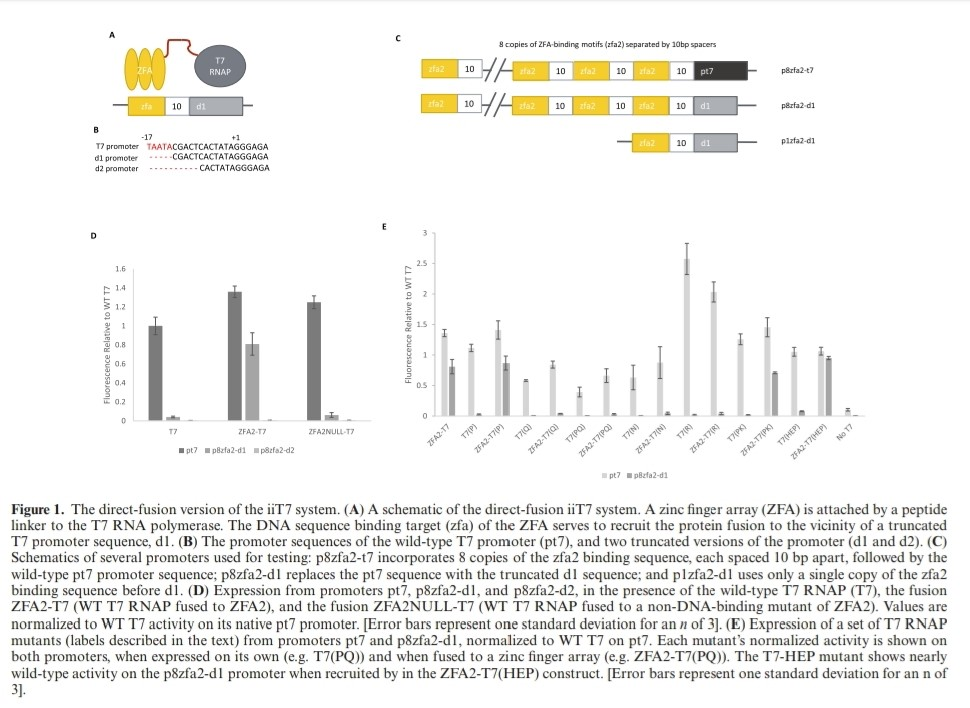
\includegraphics[width=16cm, height=12cm]{Pictures/6_1}

\paragraph{Рисунок 1.А}

Схема системы: РНК полимераза Т7 (RNAP T7) связана с блоком цинковых пальцев (ZFA), который присоединяется к своей цели (zfa), тем самым доставляя полимеразу к усечённому промотеру d1.

\paragraph{Рисунок 1.B}

Три разных промотера: исходный промотер для RNAP T7 и два усечённых варианта.

\paragraph{Рисунок 1.C}

Варианты всей целевой последовательности: разное количество копий цели для цинковых пальцев и разные промотеры.

\paragraph{Рисунок 1.D}

Результаты для систем T7 (только полимераза), ZFA2-T7 (Т7 с блоком цинковых пальцев типа 2) и ZFA2NULL-T7 (Т7 с блоком нерабочих цинковых пальцев) для 3 типов целей: pt7 (промотер Т7), p8zfa2-d1 (8 копий цели для пальцев и усечённый промотер d1) и p8zfa2-d2 (8 копий цели для пальцев и усечённый промотер d2). Исходный промотер даёт слишком высокую вероятность транскрипции для полимеразы самой по себе, а с d2 транскрипция почти не идёт, поэтому был выбран d1.

\paragraph{Рисунок 1.E}

Разные мутации РНК полимеразы Т7: была выбрана (HEP), т.к. скорость для исходного промотера с цинковыми пальцами и без одинаковая, а для цели очень сильно отличается.

\subsubsection{Рисунок 2}

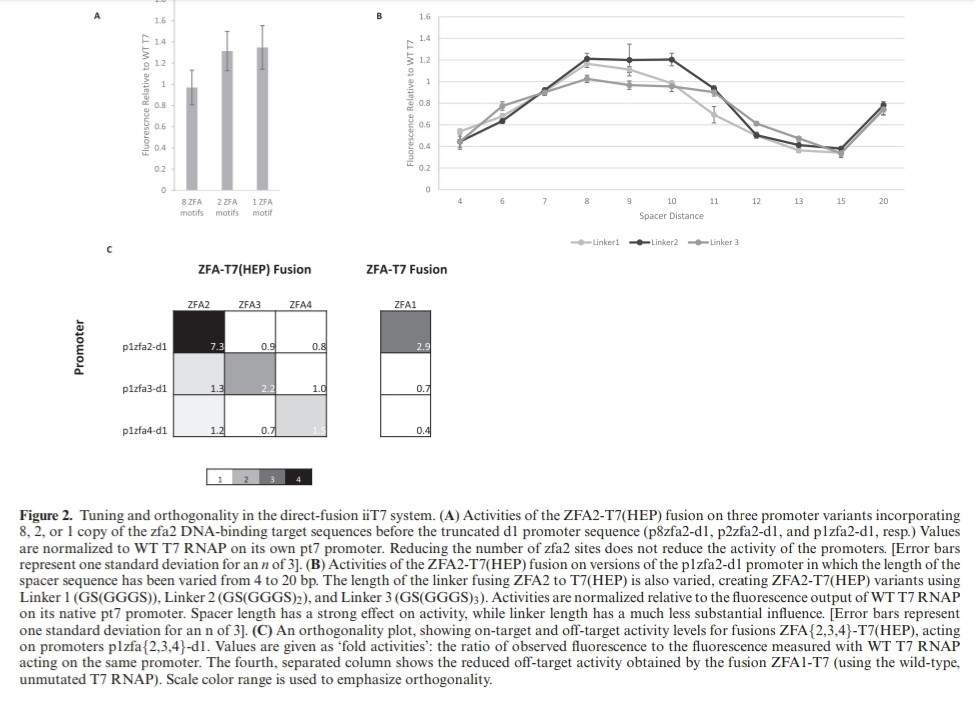
\includegraphics[width=16cm, height=12cm]{Pictures/6_2}

\paragraph{Рисунок 2.А}

Зависимость величины эффекта для ZFA2-T7(HEP) от количества копий цели для цинковых пальцев zfa2: 8 копий дают плохой результат, 2 или 1 лучше.

\paragraph{Рисунок 2.B}

Зависимость от длины связи между полимеразой и цинковыми пальцами (3 линии разного цвета) и размера промежутков в целевой последовательности.


\paragraph{Рисунок 2.С}

Таблица результатов для проверки ортогональности: ортогональность достаточно слабая, но в некоторой мере присутствует.

\subsubsection{Рисунок 3}

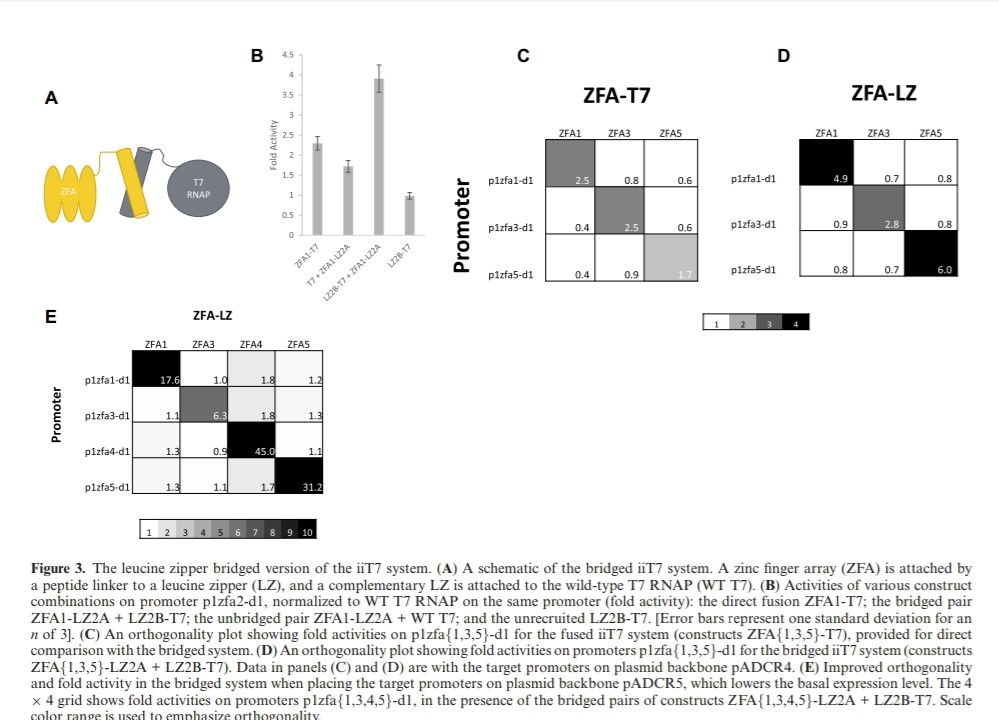
\includegraphics[width=16cm, height=12cm]{Pictures/6_3}

\paragraph{Рисунок 3.А}

Схема системы с лейциновым мостиком: цинковые пальцы ZFA5 дали слишком сильную связь, которая не разрывалась полимеразой, и транскрипция после доставки к цели не начиналась. В данном варианте мостик должен разорваться и транскрипция должна начаться.

\paragraph{Рисунок 3.B}

Относительная частота транскрипции для систем с цинковыми пальцами; с цинковыми пальцами, к которым присоединена половина мостика; с мостиком; без цинковых пальцев с половиной мостика на полимеразе.

\paragraph{Рисунки 3.C, 3.D и 3.Е}

Сравнение ортогональности - без мостика (С), с мостиком (D) и с мостиком с заменой плазмида-основы с pADCR4 на pADCR5 (E) (про что в статье ничего, кроме подписи к рисунку, нет). Итог, Е, показывает хорошую ортогональность и силу эффекта.


